\chapter{Hardware}

\begin{goals}
\item Know the major components which make up computer systems.
\item Know some examples of input and output devices, and understand their importance.
\item Understand the difference between main memory and secondary memory.
\item Learn the importance of the CPU.
\end{goals}

This chapter will focus on \emph{hardware}, the physical devices that work together to perform a common task (or tasks).  When most of us think about computers, we often think of a desktop or laptop computer, equipped with a keyboard, mouse, and monitor as seen in Figure~\ref{fig:hardware:computers}. However, many things we interact with daily are computerized, including cell phones, cars, traffic lights, smart watches, televisions, and manufacturing lines. Each of these items has sensors to perceive the real world, uses an embedded computing device to understand the sensory input, and uses a combination of display and mechanical devices to interact with the real world. Thus, each of these commonplace items contain computer hardware that is essential to their operation.

\begin{figure}
	\centering
	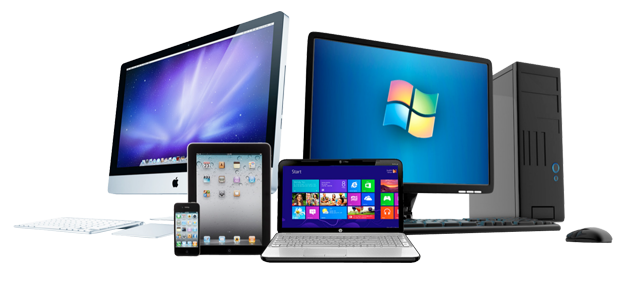
\includegraphics[width=0.85\textwidth]{images/computer_system.png}
	\caption{A variety of computer systems: desktops, a laptop, a tablet, and a
    smart phone. \afm{Source for pic.}}
	\label{fig:hardware:computers}
\end{figure}

\begin{example}\label{exmp:traffic_light}
  For intersections across busy roadways, some traffic lights are computerized to optimize road traffic. These lights will stay green along the busier of the two roads, and use cameras or pressure sensors to detect the presence of cars along the less busy of the two roads. When cars arrive, the lights switch, allowing the cars on the less busy road to cross.
\end{example}

Today we will introduce three fundamental parts of computer hardware: input and output devices, memory, and the central processing unit (CPU). These components work together to perform the basic building blocks of input processing, storage, control, and output. Ultimately, they create powerful information processing tools. We will introduce each of these parts in turn. In Figure~\ref{fig:hardware:overview}, we see how these parts come together to form a computer system.

\begin{figure}
	\centering
	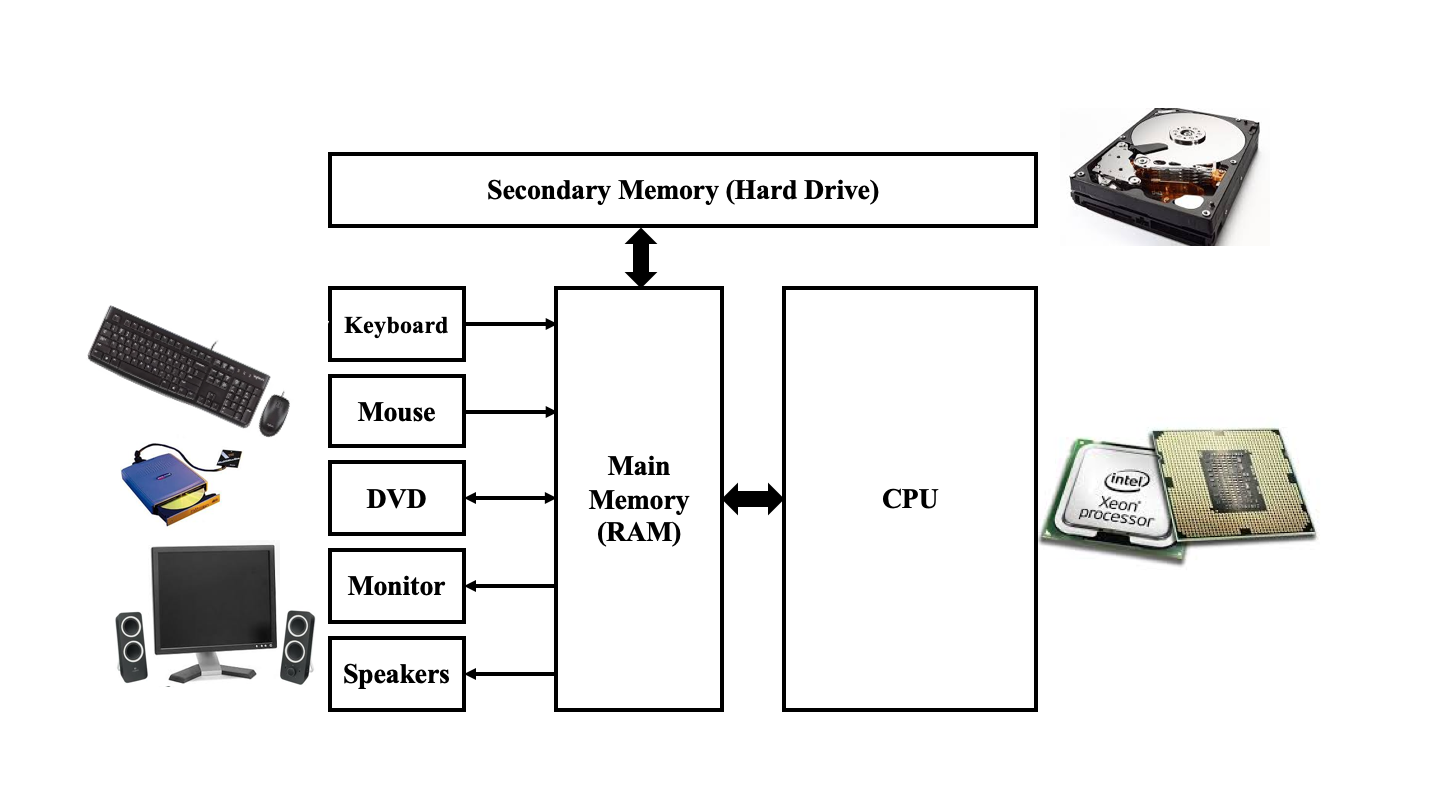
\includegraphics[width=\textwidth]{images/cs_intro_hardware_overview.png}
	\caption{Input and output devices can communicate with a computer's memory, and the memory instructs the CPU to carry out computations. Read on to learn more about each component.
                 \afm{source for pic}}
	\label{fig:hardware:overview}
\end{figure}

\section{Input and Output Devices}

Input and output  devices allow the computer to interact with users and the world directly.  \emph{Input} devices are used to bring data into the computer system. Examples include keyboards, mice, and microphones. \emph{Output} devices are used to display the results or information of a computer system. The most common forms of output are text, graphics, and sound. Examples of output devices include monitors, printers, and speakers. 

Input and output devices are essential for computer use. The computer itself can only perform computations on data stored within its memory, which we will discuss later. In order to tell the computer what to do, and what data to work with, input devices are required. In order for the user to retrieve the results of a computation, output devices are required.

For computer systems other than personal laptops and desktops, input and output devices can be even more important. For example, a modern smartphone comes equipped with a wide variety of input devices, ranging from a fingerprint scanner for authorization to an accelerometer to detect motion. In Example \ref{exmp:traffic_light}, we noted that many traffic lights contain computer systems; in this instance, there is a very important output device: the traffic light itself!

% With input and output devices, a user's input will be processed, some computations will be performed, and then the resulting output will be displayed to the user. Without these devices, a computer system would be very boring, always performing the same computation each time it's used. Even if it did compute a different value we would be unable to examine the value. A computer needs to be able to accept input and output a result. The first computers would occupy a large room in an office building and connect to a terminal (a keyboard and a text screen) in another room for users to interact with. Thanks to the hard work of electrical engineers, computers can now fit in the palm of your hand while being much more powerful. Likewise, many more types of input and output devices are now available. We still have the keyboard and monitor, and the mouse was invented for interacting with graphical displays. Today's phones are more computer than phone, coming equipped with speakers, microphones, touch screens, cameras, fingerprint scanners, radio transmitters, and much more. Computers even come embedded in other devices like cars, traffic lights, X-ray machines, and thermostats to both control and monitor the devices. As shown in Figure~\ref{fig:hardware:overview}, these devices connect to the rest of the computer through the computer's memory. This kind of input and output is called memory mapped I/O (input and output).

% Creators of input (or output) devices are assigned a section of the computer’s memory to write (for input devices) or read (for output devices) data. For example, a keyboard might write data about each key that is pressed to a given location. The computer will then read the data in that location to communicate with the keyboard. In the case of an output device, the process works in reverse: the computer writes the data in the assigned location, which the output device then reads. The creators of these devices agree on a known format to read and write data.

% You can think of communication between devices and a computer as similar to leaving messages for a friend in a locker. Only you and your friend have access to this locker, which only holds space for one message. The format you agree upon is which language you'll use to speak (e.g. English) and any special keywords or phrases. For example, you might agree upon a convention like the kind used in radio communication, where one person waits until they get an ``Over'' signal before responding with a new message. The format that devices and computers communicate in are generally very simple and structured to permit fast and easily understandable communication for computers and devices.

\begin{example}
A monitor is a graphical display for computers. Let's consider a monitor connected to a computer that only displays in black and white images that are 20 $\times$ 20 pixels large. \safemarginnote[-4cm]{This is a simplified example, but it is similar to how modern graphical displays communicate with computers.} The monitor and keyboard agree upon using the following format to communicate: the format is black and white images that are 20 $\times$ 20 pixels large. Each pixel's value is represented at 0 for black and 1 for white. Then an image is represented as a 400 = (20 $\times$ 20) long sequence of pixel values. The sequence is ordered left to right, top to bottom. Now that both the monitor and computer agree upon the communication format, the computer can write images to the section of memory dedicated to the monitor and the monitor will read the image and display the image on its screen. Figure~\ref{fig:hardware:monitor_image} displays an example image, a  20 $\times$ 20 checkerboard with its encoding. 
\end{example}

\begin{figure}%
	\centering%
	\begin{minipage}{0.45\linewidth}%
		
\includegraphics[width=\textwidth]{images/checkered_image.jpg}
	\end{minipage}%
	\hspace{.1\linewidth}%
        \begin{minipage}{0.45\linewidth}%
		\scriptsize
\begin{verbatim}
0 1 0 1 0 1 0 1 0 1 0 1 0 1 0 1 0 1 0 1
1 0 1 0 1 0 1 0 1 0 1 0 1 0 1 0 1 0 1 0
0 1 0 1 0 1 0 1 0 1 0 1 0 1 0 1 0 1 0 1
1 0 1 0 1 0 1 0 1 0 1 0 1 0 1 0 1 0 1 0
0 1 0 1 0 1 0 1 0 1 0 1 0 1 0 1 0 1 0 1
1 0 1 0 1 0 1 0 1 0 1 0 1 0 1 0 1 0 1 0
0 1 0 1 0 1 0 1 0 1 0 1 0 1 0 1 0 1 0 1
1 0 1 0 1 0 1 0 1 0 1 0 1 0 1 0 1 0 1 0
0 1 0 1 0 1 0 1 0 1 0 1 0 1 0 1 0 1 0 1
1 0 1 0 1 0 1 0 1 0 1 0 1 0 1 0 1 0 1 0
0 1 0 1 0 1 0 1 0 1 0 1 0 1 0 1 0 1 0 1
1 0 1 0 1 0 1 0 1 0 1 0 1 0 1 0 1 0 1 0
0 1 0 1 0 1 0 1 0 1 0 1 0 1 0 1 0 1 0 1
1 0 1 0 1 0 1 0 1 0 1 0 1 0 1 0 1 0 1 0
0 1 0 1 0 1 0 1 0 1 0 1 0 1 0 1 0 1 0 1
1 0 1 0 1 0 1 0 1 0 1 0 1 0 1 0 1 0 1 0
0 1 0 1 0 1 0 1 0 1 0 1 0 1 0 1 0 1 0 1
1 0 1 0 1 0 1 0 1 0 1 0 1 0 1 0 1 0 1 0
0 1 0 1 0 1 0 1 0 1 0 1 0 1 0 1 0 1 0 1
1 0 1 0 1 0 1 0 1 0 1 0 1 0 1 0 1 0 1 0
\end{verbatim}
    \end{minipage}%
	\caption{An example checkered image and its encoding, with newlines and spaces added for readability.}
	\label{fig:hardware:monitor_image}
\end{figure}

\section{Memory}

Quick: what's $347 \times 782$? Did you feel yourself reach for a piece of scratch paper? Computers may be faster than humans at calculations, but they still have to go step by step and keep track of their work as they go. This means that computers need a form of scratch paper, too. They also need a more long-term storage mechanism, for saving data that a user might need to work with more at a later date. This is more like your course notebook than a piece of scratch paper: a place where you write things down that you may need to come back to weeks or months from now.\marginnote{271354, if you were wondering.}

Both of these types of storage systems form parts of a computer's \emph{memory}. The ``scratch paper'' form of memory is called \emph{main memory}, or RAM\marginnote{RAM stands for Random Access Memory. The term ``random access'' means that the computer can access it at any location -- it doesn't have to slowly scan through to find the correct point at which to read.}. The long term memory is called secondary memory, and in modern computers typically takes the form of a hard drive or solid state drive.

There is a key tradeoff between the two types of memory. As we've mentioned, secondary memory is meant for long term storage. It is designed to be \emph{persistent}, also known as \emph{nonvolatile}, meaning that data stored in secondary memory is safe for long periods of time. In particular, it does not go away when the computer is turned off. The cost of this persistence is that it takes longer for the computer to read and write from secondary memory. Think about your scratch paper and your course notebook: it takes longer to find the right location in your notebook to write something and to write it out nicely, but the benefit is that you'll be able to access that information far in the future.

Main memory has the opposite combination: it is volatile, meaning it is not preserved when the computer turns off. The computer effectively has to throw its scratch paper away every time it goes to bed. However, reading and writing from main memory can happen very quickly. This is why it is used to store the intermediate results of calculations: the calculations go much more quickly if they use main memory instead of secondary memory.

Memory is also home to a very special kind of data: computer programs. The step-by-step instructions which form a program can be stored safely in secondary memory. When it is time to run a program, its instructions are loaded into main memory so that it can be run rapidly. The program might instruct the computer to save some of the results of a computation to secondary memory, so that they can be accessed later on.

% \begin{figure}
% 	\centering
% 	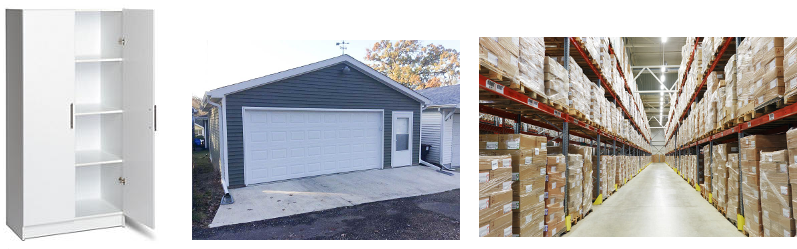
\includegraphics[width=0.85\textwidth]{images/storage.png}
% 	\caption{Storage closet, garage, and warehouse trading off between
%                  capacity and locality. \afm{picture references}}
% 	\label{fig:hardware:storage}
% \end{figure}

\section {Central Processing Unit}

The final part of a computer we will introduce today is the \emph{central processing unit} (CPU), also known as the \emph{processor} or \emph{main processor}. The CPU is the physical circuitry of a computer that performs instructions. This is where all the magic happens.

The CPU is divided into several components. It has an arithmetic and logic unit (ALU) which is responsible for physically carrying out basic mathematical operations. It also has control logic which helps the CPU to determine which instructions to carry out. One especially important component of the CPU is its clock, which keeps track of how many steps, known as ``clock cycles,'' the CPU has carried out.

The CPU has several key components: the control logic, arithmetic and logic unit (ALU), registers, program counter, and clock. These components work together to 
fetch, decode, and execute all instructions --- the building blocks of all programs. Instructions vary between different brands of CPUs, but, in general, they will include arithmetic, control, read (from memory), and write (to memory) functionalities.\marginnote{A typical computer today might run at 2.4 GHz -- which means its clock goes through 2.4 billion cycles every second. That's fast!}

We already discussed how a computer uses its main memory as scratch paper. Even when you use scratch paper, though, you do a little bit of arithmetic -- things like adding two one-digit numbers -- in your head. Your head is like your CPU, and it has to be able to store those few numbers so you can work with them. When a CPU does math ``in its head,'' it uses special memory locations called registers. Most modern CPUs will have between 16 and 64 registers that programs may use. That may not sound like a lot, but imagine trying to hold 64 numbers in your head at once!

In most computers, the CPU and its constituent parts are responsible for all computing needs of the computer. \marginnote{In some select systems, there will be additional hardware to perform specialized operations. For example, graphics processing units are specialized for producing images.} It is the CPU's responsibility to control the computer and coordinate with devices to execute programs. Since it is so important, lots of effort has gone towards increasing the processing power of the CPU. Electrical engineers originally focused on making the CPU smaller and smaller, which results in it running more quickly. The evolution followed a trend called Moore's Law: every two years the size of a CPU would be reduced by a factor of two.

CPUs have become so small that it is difficult to shrink them further. However, engineers have still been able to increase the processing power of computers by building CPUs which have multiple copies of the core components that can work together to run different instructions at the same time. Programmers refer to this behavior as \emph{parallelism}. In a future class, you may learn how to write programs which can run in parallel.


\section {Conclusion}

In this chapter, we covered the three fundamental parts of a computer system: input and output devices, main and secondary memory, and the CPU. We discussed their roles, relationships, and basic capabilities. This will help you better understand how hardware works, so that you understand what is happening when you write programs that will eventually run on these computer systems. In the next chapter we will begin discussing the concept of software and how it interacts with hardware to make computers work.

\exercisesection

\begin{exercise}
What three parts comprise a computer system?
\end{exercise}

\begin{exercise}
What are examples of common input and output devices?
\end{exercise}

\begin{exercise}
What are some components of a CPU?
\end{exercise}

\begin{exercise}
Explain the difference between main and secondary Memory.
\end{exercise}
